\documentclass[11pt,a4paper]{article}
\usepackage[T1]{fontenc}
\usepackage{lmodern}
\usepackage[margin=2.3cm]{geometry}
\usepackage{booktabs}
\usepackage{tabularx}
\usepackage{array}
\usepackage{graphicx}
\usepackage{xcolor}
\usepackage{enumitem}
\usepackage{amsmath}
\usepackage{caption}
\usepackage{tikz}
\usetikzlibrary{positioning,arrows.meta,shapes}
\usepackage[hidelinks]{hyperref}
\usepackage{fancyhdr}

\definecolor{accent}{HTML}{1F5A85}
\definecolor{soft}{HTML}{EEF3F8}
\hypersetup{colorlinks=true,linkcolor=accent,urlcolor=accent}
\setlist{itemsep=2pt,topsep=4pt}
\setlength{\parskip}{4pt}
\setlength{\parindent}{0pt}
\renewcommand{\arraystretch}{1.25}
\newcolumntype{L}{>{\raggedright\arraybackslash}X}
\pagestyle{fancy}
\fancyhf{}
\lhead{\small GBST + BERT on human DNA}
\rhead{\small Report, 7 October 2026}
\cfoot{\small\thepage}

\newcommand{\code}[1]{\texttt{\small #1}}

\begin{document}
\sloppy

\begin{center}
{\LARGE\bfseries\color{accent} A ChaRNABERT-style model for human DNA}\\[6pt]
{\large GBST tokenization + bidirectional BERT encoder, on the DNA-xLSTM code base}\\[10pt]
Report \quad$\cdot$\quad Omar R.A Mohamed \quad$\cdot$\quad 7 October 2026\\[4pt]
Code: \url{https://github.com/OMAR622-ai/dna-xlstm-charna} (branch \code{charna-gbst}, private)
\end{center}

\vspace{4pt}
\noindent\colorbox{soft}{\parbox{\dimexpr\linewidth-2\fboxsep}{
\textbf{Summary.} The ChaRNABERT architecture --- a learnable tokenizer (GBST) in front of a
bidirectional BERT encoder --- was implemented in the DNA-xLSTM code base, tested (24 automatic
tests) and trained on 10.5 billion bases of the human genome (hg38) with the DNA-xLSTM protocol.
On unseen test DNA, the final model guesses \textbf{56.4\%} of hidden bases correctly (random
guessing 25\%, always the most common base 29.4\%), with a loss of \textbf{0.975} --- in the range
of the published 2\,M DNA models. A same-size model without GBST (Transformer++) reached 56.3\% and
0.977: GBST-BERT was ahead during most of the training but only 0.1 percentage points at the end,
too little to call GBST better after one run each. Inside the model, GBST learned to put about
98\% of its weight on single bases, so on human DNA it behaves almost like reading one base at a
time. No benchmark (downstream task) results yet.
}}

\tableofcontents
\vspace{6pt}

% ------------------------------------------------------------------------------------------
\section{Goal}

The project asks whether a \emph{learned} way of reading DNA helps a small model. ChaRNABERT
(Morales-Pastor et al., 2024) showed this for RNA. We take its architecture, train it on the human
genome with the short-context protocol of the DNA-xLSTM paper (Schmidinger et al., 2024), and
compare it with models from that paper. The plan has three parts: (1) pretraining on hg38 with
masked language modelling; (2) evaluation on held-out DNA (accuracy and loss); (3) later, the
18-task Nucleotide Transformer (NT) benchmark. Parts (1)--(2) are done; part (3) is ready but
postponed.

% ------------------------------------------------------------------------------------------
\section{How the ChaRNABERT model works}

ChaRNABERT is an RNA ``foundation model'' from Nostrum Biodiscovery (arXiv:2411.11808). Its name
combines \emph{Cha}racter (single letters), \emph{RNA} and \emph{BERT}. Its central idea: most
models fix in advance how a sequence is cut into ``words'' (single bases, codons, k-mers);
ChaRNABERT lets the model \textbf{learn how to cut, separately at every position}.

\begin{center}
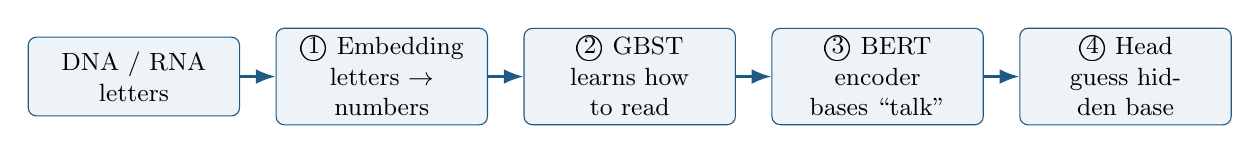
\begin{tikzpicture}[
  box/.style={draw=accent, rounded corners=3pt, fill=soft, minimum height=1.0cm, align=center, font=\small, text width=2.45cm},
  arr/.style={-{Latex[length=2.5mm]}, thick, accent}]
\node[box] (in) {DNA / RNA\\letters};
\node[box, right=0.45cm of in] (emb) {\textcircled{1} Embedding\\letters $\to$ numbers};
\node[box, right=0.45cm of emb] (gbst) {\textcircled{2} GBST\\learns how to read};
\node[box, right=0.45cm of gbst] (enc) {\textcircled{3} BERT encoder\\bases ``talk''};
\node[box, right=0.45cm of enc] (head) {\textcircled{4} Head\\guess hidden base};
\draw[arr] (in) -- (emb); \draw[arr] (emb) -- (gbst); \draw[arr] (gbst) -- (enc); \draw[arr] (enc) -- (head);
\end{tikzpicture}
\end{center}

\textbf{\textcircled{1} Embedding --- letters become numbers.} Each letter is replaced by a learned
list of numbers (256 in our model), like a profile describing that nucleotide.

\textbf{\textcircled{2} GBST (Gradient-Based Subsequence Tokenization) --- learning how to read.}
\begin{enumerate}
\item \emph{Smooth}: each base is mixed a little with its neighbours (a short filter).
\item \emph{List candidates}: at every position, every block of 1, 2, 3 or 4 bases that contains
  the position. Blocks of the same size start at different places, like reading frames
  (``offsets''). This gives 10 candidates per position (Table~\ref{tab:gbst}).
\item \emph{Score}: a small learned scorer rates each candidate (``how useful is this reading
  here?''); the scores become weights that add up to 1.
\item \emph{Make the choice consistent}: positions with similar weight patterns pull towards
  each other, so the ``reading style'' is consistent along the sequence (ChaRNABERT Eq.~6).
\item \emph{Blend}: each base's output is the weighted mix of its 10 candidates. There is one
  output per base --- ChaRNABERT removes Charformer's shortening step, because many tasks need
  single-base detail.
\end{enumerate}
Biology analogy: a ribosome reads triplets, a transcription factor a 6--10-base motif, a methylase
CpG pairs. GBST can learn to read ``like a ribosome'' in one place and ``like a methylase'' in
another, without being told which.

\begin{table}[h]
\centering
\caption{The 10 GBST candidates for position 3 (the first T) of \code{ACGTTGCA}.}
\label{tab:gbst}
\small
\begin{tabular}{cl}
\toprule
Block size & Candidate blocks that contain position 3 \\
\midrule
1 & \code{T} \\
2 & \code{TT} (positions 3--4), \code{GT} (2--3) \\
3 & \code{TTG} (3--5), \code{GTT} (2--4), \code{CGT} (1--3) \\
4 & \code{TTGC} (3--6), \code{GTTG} (2--5), \code{CGTT} (1--4), \code{ACGT} (0--3) \\
\bottomrule
\end{tabular}
\end{table}

\textbf{\textcircled{3} BERT encoder --- bases talk to each other.} A stack of identical blocks
(4 in our model). In each block, \emph{attention} lets every base gather information from every
other base, in both directions (\emph{bidirectional}); then a small \emph{feed-forward} network
processes each position. The paper adds RoPE (encodes distances between bases), QKNorm (keeps
training stable), SwiGLU (a better feed-forward type) and FlashAttention~2 (faster attention).

\textbf{\textcircled{4} Prediction head.} For every position, a score for each possible letter.

\textbf{Learning: the fill-in-the-blank game.} In \emph{pretraining}, 15\% of the bases are hidden
and the model must guess them from the context (\emph{masked language modelling}, MLM). To do this
well it must learn motifs, codon patterns, pairing rules --- without any labels. The paper also
tested \emph{UL2}, which additionally hides longer stretches. ChaRNABERT was trained on 62 million
RNA sequences (31 M non-coding from RNAcentral, 31 M coding from RefSeq), with models of 8 M to
650 M parameters. Afterwards it is \emph{fine-tuned} on specific labelled questions.

\textbf{What the paper found.} GBST gave a lower loss than single-letter reading in most settings
(e.g.\ 0.498 vs.\ 0.508 for the 5 M model, Table~2); performance saturated around 30--50 M
parameters; the 8 M model matched or beat much larger models on several tasks, e.g.\ RNA--protein
binding F1 0.833 vs.\ 0.831 for the 650 M RiNALMo (Table~5).

% ------------------------------------------------------------------------------------------
\section{How we apply ChaRNABERT to DNA}

\textbf{The model stays the same; the data and the setting change.}

\begin{enumerate}
\item \textbf{DNA instead of RNA.} The human genome hg38 (about 3 billion letters), in pieces of
  1,024 bases. Alphabet A, C, G, T (N = unknown, ignored).
\item \textbf{Letters to numbers.} A\,=\,7, C\,=\,8, G\,=\,9, T\,=\,10 (the repository's tokenizer).
\item \textbf{The same game.} 15\% of the bases are hidden and must be guessed; with 50\%
  chance the reverse-complement strand is shown instead, so the model learns that both strands
  are equivalent.
\begin{center}\small
\begin{tabular}{ll}
Real:   & \code{A C G T T G C A A G T C} \\
Input:  & \code{A C ? T T G C A A ? T C} \\
Answer: & \code{. . G . . . . . . G . .} \quad (dots: not hidden, not graded)
\end{tabular}
\end{center}
\item \textbf{The same architecture}, GBST + BERT encoder, but small: 2.1 million parameters, the
  size of the DNA-xLSTM paper's models, so the comparison is fair.
\item \textbf{Train, test, compare.} Train on millions of DNA pieces; test on DNA never seen in
  training (accuracy of the guesses); compare with the same encoder \emph{without} GBST
  (Transformer++). If ours guesses better, GBST helps on DNA.
\end{enumerate}

\begin{table}[h]
\centering
\caption{ChaRNABERT paper vs.\ this project.}
\small
\begin{tabularx}{0.9\linewidth}{lLL}
\toprule
 & ChaRNABERT paper & This project \\
\midrule
Data & RNA (RNAcentral, RefSeq) & Human DNA (hg38) \\
Letters & A, C, G, U & A, C, G, T \\
Model & GBST + BERT & GBST + BERT (same) \\
Training game & Guess hidden bases (MLM; UL2 tested) & Same (MLM; UL2 available as an option) \\
Model size & 8 M -- 650 M parameters & 2.1 M (to compare with DNA-xLSTM) \\
Piece length & up to 8,190 bases & 1,024 bases (DNA-xLSTM protocol) \\
Later tasks & BEACON RNA benchmark & Nucleotide Transformer DNA benchmark \\
\bottomrule
\end{tabularx}
\end{table}

% ------------------------------------------------------------------------------------------
\section{What was done, step by step}

\begin{enumerate}[leftmargin=*]
\item \textbf{Read the code base and the four papers} (Bio-xLSTM, ChaRNABERT, Charformer, UL2);
  every setting was taken from a paper table or section, or marked as our own choice.
\item \textbf{Server set-up.} JKU server \code{student01}: 4$\times$ NVIDIA GTX 1080 Ti, shared with
  another user. Installed a Python environment that works on these older GPUs (PyTorch 2.2 +
  CUDA 12.1); newer PyTorch versions no longer support them. Copied the genome (3.1 GB) and checked
  it with an md5 checksum. Set up key-based SSH login.
\item \textbf{Implemented the model} (\code{models/charna/}): GBST (\code{gbst.py}), the
  bidirectional encoder and prediction head (\code{modeling\_charna.py}), settings
  (\code{configuration\_charna.py}), and registered it in the training program. Existing models
  behave exactly as before.
\item \textbf{Implemented UL2 masking} as an option (\code{src/dataloaders/utils/ul2.py}).
\item \textbf{A launcher} (\code{scripts\_charna/train\_charna.py}) so the repository's training
  program runs on GPUs that cannot install two optional packages (mamba\_ssm, flash\_attn).
\item \textbf{Scripts}: pretraining (\code{run\_pretrain\_charna.sh}), benchmark fine-tuning,
  results table, loss plot, accuracy evaluation (\code{evaluate\_mlm.py}), data download with
  checksum, a small genome sample for GitHub, result collection.
\item \textbf{Tests}: 23 automatic tests (Section~\ref{sec:results}); a check that the model can
  memorise one batch; a 3-step trial on 4 GPUs; a 48-step smoke run of both models.
\item \textbf{Matched the paper exactly} where possible (after review on 4 October): added the
  ``pointwise'' layer that ChaRNABERT's parameter table (Table~9) implies; switched the learning
  rate to ChaRNABERT's 5e-4 (Table~2); restored UL2 as an option.
\item \textbf{Bugs found and fixed}: (a) loading pretrained GBST weights into the benchmark code
  crashed; (b) the benchmark data loader mixed all 18 tasks together (461,850 examples instead
  of e.g.\ 5,509) --- a bug in the original repository caused by a change on Hugging Face; (c) a
  results file wrote values under wrong column names; (d) the GitHub genome sample first held
  only 1/8 of each region; (e) smaller script issues (wrong exit status in a log, a path error).
\item \textbf{Small experiment} (4 October): both models trained for 500 steps
  ($\approx$0.5 billion bases); then accuracy evaluation on 2,048 held-out sequences. The
  first full run was stopped to get results sooner; the benchmark was postponed.
\item \textbf{Learning-rate check} (4--5 October): four short GBST-BERT runs; 2e-3 was best.
\item \textbf{Full training} (5--6 October): GBST-BERT with 2e-3, then Transformer++, 10,000 steps
  each; moved from server student01 to student07 (faster GPUs, same files) at step 3,000.
\item \textbf{Data-loading bug} (5 October): found after a crash, measured, fixed with a test;
  GBST-BERT resumed from step 3,000, Transformer++ restarted.
\item \textbf{Final evaluation and analysis} (6 October): accuracy of both final models; what
  block sizes GBST uses; all models saved on GitHub.
\item \textbf{Documentation and GitHub}: project README (front page), a beginner's explanation
  (\code{docs/EXPLAINED.md}), 50 questions and answers (\code{docs/QA\_50.md}), one page per run
  (\code{charna\_project/runs/}), everything in one folder (\code{charna\_project/}: code, data
  that fits in git, models, results), and this report.
\end{enumerate}

\textbf{Main settings} (all for GBST-BERT; source in brackets):
\begin{center}\small
\begin{tabularx}{0.95\linewidth}{lL}
\toprule
Model & 256 numbers per base, 4 encoder blocks, 8 attention heads, 2,107,392 parameters [Bio-xLSTM Table A3] \\
GBST & blocks of 1--4 bases with offsets, sum pooling, calibration, no shortening [ChaRNABERT \S3.2] \\
Masking & 15\% of bases; of these 80\% \code{[MASK]}, 10\% random, 10\% unchanged [Bio-xLSTM App.~C.5] \\
Batch & 1,024 sequences $\times$ 1,024 bases = 1,048,576 bases per step [Bio-xLSTM App.~C.5] \\
Learning rate & 2e-3, best of 5e-4 [ChaRNABERT Table 2], 1e-3, 2e-3, 5e-3 in a short check; warmup 10\% of steps, cosine decay [Bio-xLSTM Table A4] \\
Optimizer & AdamW, $\beta=(0.9, 0.95)$, weight decay 0.1 [Bio-xLSTM Table A4] \\
Length of training & small experiment 500 steps (0.5 B bases); full run 10,000 steps (10.5 B) \\
Comparison model & Transformer++-2M, learning rate 1e-2 [Bio-xLSTM Table A3] \\
\bottomrule
\end{tabularx}
\end{center}

% ------------------------------------------------------------------------------------------
\section{Results}
\label{sec:results}

\textbf{Automatic tests: 23 of 23 pass.} They check, among others, that GBST matches a slow
reference implementation of the paper's equations, that it has the weight count of the paper's
Table~9, that the model looks in both directions, that the loss counts only hidden bases, that
about 15\% of bases are hidden, that UL2 never leaks the answer, and that pretrained weights load
correctly into the benchmark code.

\textbf{Memorising one batch: passed.} The loss fell below 0.05 after 164 steps (MLM) and 230
steps (UL2), so the model is able to learn.

\textbf{Smoke run} (48 steps, 50 million bases, an earlier GBST version with learning rate 1e-2).
Loss is in nats per hidden base; 1.386 = random guessing among 4 bases.

\begin{center}
\begin{minipage}{0.42\linewidth}\small
\begin{tabular}{rcc}
\toprule
Bases & GBST-BERT & Transformer++ \\
\midrule
13 M & 1.392 & 1.397 \\
25 M & 1.370 & 1.363 \\
38 M & 1.366 & 1.343 \\
50 M & 1.364 & 1.325 \\
\bottomrule
\end{tabular}
\end{minipage}\hfill
\begin{minipage}{0.55\linewidth}
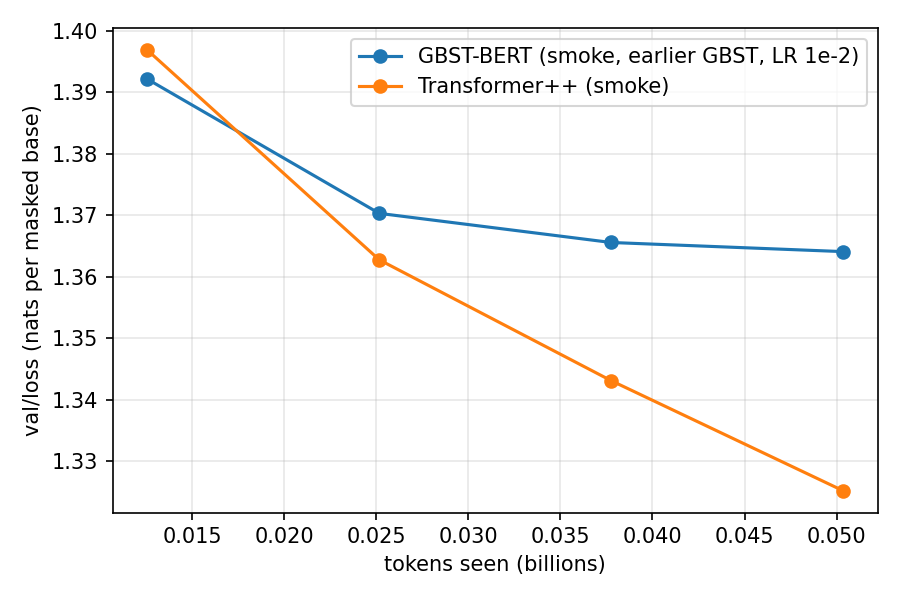
\includegraphics[width=\linewidth]{figures/smoke_val_loss.png}
\end{minipage}
\end{center}

Both models learn, but this run only checked that everything works: it was very short and used
the older GBST and learning rate. A test of the accuracy script on these smoke models showed why
accuracy needs reference values: the smoke GBST model reached 29.1\% only by always answering
``A'' (the most common hidden base), i.e.\ no better than no model; Transformer++ reached 32.8\%.

\textbf{Small experiment (finished 4 October, 22:05).} Both models trained for 500 steps
($\approx$0.52 billion bases) with the settings of Section~4. Validation loss during training
(2\% of the validation set):

\begin{center}
\begin{minipage}{0.47\linewidth}\small\setlength{\tabcolsep}{4pt}
\begin{tabular}{rccc}
\toprule
Step & Bases & GBST-BERT & Transformer++ \\
\midrule
100 & 0.10 B & 1.3399 & 1.2626 \\
200 & 0.21 B & 1.3011 & 1.2422 \\
300 & 0.31 B & 1.2146 & 1.2112 \\
400 & 0.42 B & 1.2004 & 1.1996 \\
500 & 0.52 B & \textbf{1.1944} & 1.1960 \\
\bottomrule
\end{tabular}
\end{minipage}\hfill
\begin{minipage}{0.51\linewidth}
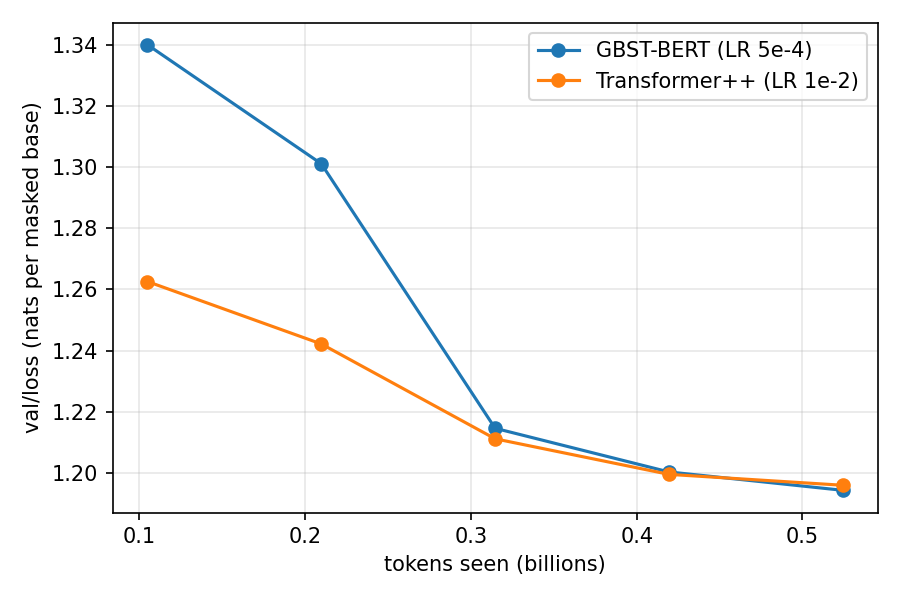
\includegraphics[width=\linewidth]{figures/small_val_loss.png}
\end{minipage}
\end{center}

\textbf{Accuracy test.} The final models predicted the hidden bases of 2,048 test sequences they
had never seen (311,767 hidden bases; both models got exactly the same hidden positions).
Validation-split values in brackets.

\begin{center}\small\setlength{\tabcolsep}{4pt}
\begin{tabular}{lcccccc}
\toprule
Model & Loss & Accuracy & A & C & G & T \\
\midrule
GBST-BERT & 1.1944 (1.1945) & \textbf{43.94\%} (44.12\%) & 53.9\% & 32.0\% & 36.1\% & 47.9\% \\
Transformer++ & 1.1958 (1.1955) & 43.77\% (43.95\%) & 51.0\% & 33.0\% & 31.5\% & 52.8\% \\
Random guess & 1.3863 & 25.00\% & 25\% & 25\% & 25\% & 25\% \\
Always ``A'' (most common) & -- & 29.42\% (29.97\%) & & & & \\
\bottomrule
\end{tabular}
\end{center}

\textbf{What this means.}
\begin{itemize}
\item \emph{Both models learned real DNA patterns}: 44\% accuracy, well above random guessing
  (25\%) and above always guessing the most common base (29--30\%); loss 1.19 versus 1.37 for a
  model that knows only the base composition.
\item \emph{GBST-BERT starts slower, then catches up}: it first has to learn \emph{how} to read
  before it can use it. At the end it is very slightly ahead (+0.17 percentage points accuracy on
  both splits). With a single training run per model, this is too small to call a winner.
\item \emph{Different strengths per base}: GBST-BERT predicts G better (36\% vs.\ 31.5\%) and T
  worse (48\% vs.\ 53\%).
\item \emph{Room to improve}: the published 2 M models reach about 0.96--1.03 test loss after
  2--10 billion bases (Bio-xLSTM Fig.~2). Both curves here are still falling at 0.5 billion bases.
\end{itemize}

\subsection*{Learning-rate check (5 October)}
ChaRNABERT's 5e-4 comes from an RNA model with another batch size, so four GBST-BERT runs with the
small-experiment setup (500 steps) were compared by \emph{validation} loss (the test split was not
used for the choice): 5e-4: 1.194, 1e-3: 1.187, \textbf{2e-3: 1.154}, 5e-3: 1.160. The full run
used 2e-3. Transformer++ kept its paper value (1e-2, Bio-xLSTM Table A3) and was not re-tuned.

\subsection*{Full training (10.5 billion bases)}
Both models trained for 10,000 steps (10.5 billion bases, about 4.5 passes over the 2.33 billion
unique training bases). Validation loss during training (12.5\% of the validation set):

\begin{center}
\begin{minipage}{0.48\linewidth}\small\setlength{\tabcolsep}{3pt}
\begin{tabular}{rccc}
\toprule
Step & Bases & GBST-BERT & Transformer++ \\
\midrule
2,000 & 2.1 B & 1.0559 & 1.0516 \\
4,000 & 4.2 B & \textbf{1.0014} & 1.0153 \\
6,000 & 6.3 B & \textbf{0.9853} & 0.9963 \\
8,000 & 8.4 B & \textbf{0.9765} & 0.9823 \\
10,000 & 10.5 B & \textbf{0.9728}$^*$ & 0.9755 \\
\bottomrule
\end{tabular}
\end{minipage}\hfill
\begin{minipage}{0.50\linewidth}
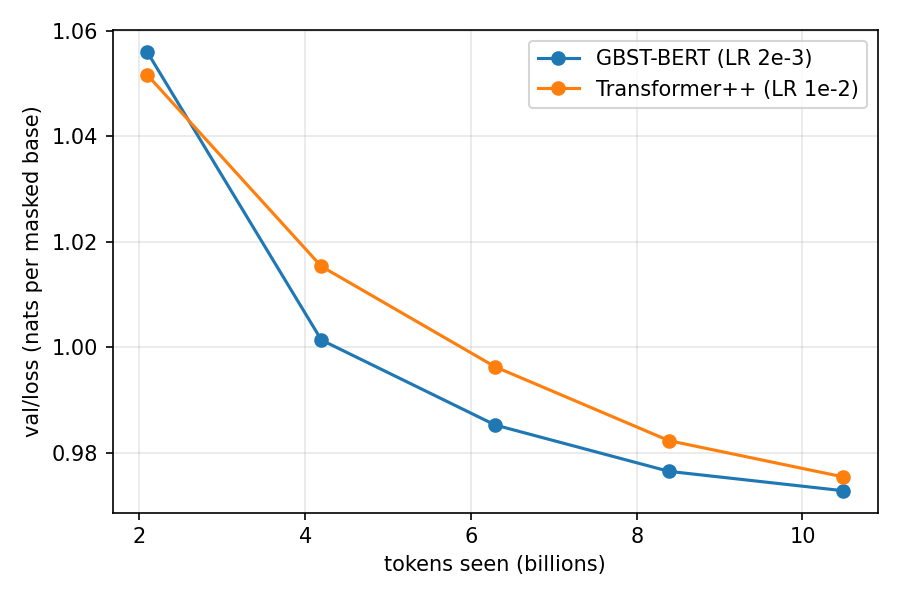
\includegraphics[width=\linewidth]{figures/full_val_loss.png}
\end{minipage}
\end{center}
$^*$ After resuming, the training program counted one step ahead, so GBST-BERT's last scheduled
check fell on step 10,001 and was skipped. It was measured afterwards on the final model with
exactly the same settings (validation 0.9728, test 0.9670).

\textbf{Final accuracy test.} Both final models predicted the hidden bases of the same 2,048
unseen test sequences (311,767 hidden bases, identical masks). Validation split in brackets.

\begin{center}\small\setlength{\tabcolsep}{4pt}
\begin{tabular}{lcccccc}
\toprule
Model & Loss & Accuracy & A & C & G & T \\
\midrule
GBST-BERT & \textbf{0.9753} (0.9689) & \textbf{56.44\%} (56.80\%) & 61.8\% & 48.5\% & 48.8\% & 62.1\% \\
Transformer++ & 0.9774 (0.9728) & 56.33\% (56.65\%) & 61.3\% & 48.9\% & 48.9\% & 61.9\% \\
Random guess & 1.3863 & 25.00\% & 25\% & 25\% & 25\% & 25\% \\
Always ``A'' (most common) & -- & 29.42\% (29.97\%) & & & & \\
\bottomrule
\end{tabular}
\end{center}

\subsection*{What GBST learned}
Measured on 8 sequences from different chromosomes, the share of GBST's weight on blocks of
1 / 2 / 3 / 4 bases was 72 / 22 / 5 / 1\% after 500 steps at learning rate 5e-4, but
98 / 2 / 0 / 0\% at 2e-3 and \textbf{98 / 2 / 0 / 0\% in the final model}. On human DNA, GBST thus
learned to read almost only single bases (each still mixed with its neighbours by the
convolution before the blocks).

\subsection*{A data-loading bug, found and fixed}
On 5 October the full GBST-BERT run crashed when the data loader returned an empty sequence.
Cause: in the repository's genome reader, the parallel reader processes shared one open file and
its read position, so they sometimes read the wrong bases. Measured: 0.35\% of sequences with 2
readers per GPU (all runs on the first server), 13--33\% with 12. Wrong reads stayed within their
data split (no test DNA in training), and the accuracy tests read without parallel readers. The
file is now opened separately in each reader (with a test: 841 of 1,024 sequences wrong without the
fix, 0 with it); GBST-BERT was resumed from its last checkpoint before the problem (step 3,000) and
Transformer++ was trained from scratch with the fix.

\subsection*{Conclusions}
\begin{itemize}
\item Both 2\,M models learned human DNA well (56\% accuracy, loss $\approx$0.975), in line with
  the published models of the same size.
\item GBST-BERT was ahead for most of the training, but at the end the difference is 0.1
  percentage points --- too small to say that GBST helps, with one run per model.
\item GBST learned to use mostly single bases, which explains why the two models end so close.
\item Not fully controlled: only GBST-BERT's learning rate was tuned, and the two models also
  differ in normalization. The same model with GBST replaced by a plain lookup table would
  isolate the effect of GBST.
\end{itemize}

% ------------------------------------------------------------------------------------------
\section{Differences from the papers}

\begin{center}\small
\begin{tabularx}{\linewidth}{>{\raggedright\arraybackslash}p{4.3cm}>{\raggedright\arraybackslash}p{3.4cm}L}
\toprule
Paper & This project & Reason \\
\midrule
FlashAttention 2, bf16 numbers & standard attention, fp32 & Our GPUs (GTX 1080 Ti, RTX 2080 Ti, Quadro GV100) support neither; the result is the same, only slower \\
Eq.~3: offsets written as $X_{i+o:i+o+b}$ & blocks that contain position $i$ & Read literally, a position would get blocks that do not include it; the text (reading frames) describes our version \\
Eq.~9: SwiGLU written as $\sigma(xW_1)\odot\text{swish}(xW_2)$ & standard SwiGLU & The text cites the standard SwiGLU; the printed formula is a different function \\
Eq.~1: depthwise convolution & + a $256\times256$ pointwise layer & The paper's Table~9 counts $d\cdot M + d^2$ weights, which implies it \\
Maximum block size not stated & 4 & As in Charformer's figure (our choice) \\
RNA, 2--8 k bases, 8--650 M parameters & DNA, 1,024 bases, 2 M & Comparability with DNA-xLSTM (project plan) \\
Repository Transformer++ script: LR 8e-3, hidden size 1,024 & LR 1e-2, hidden size 320 & We follow the Bio-xLSTM paper's Table A3 \\
\bottomrule
\end{tabularx}
\end{center}

\textbf{Uncertain points:} the block size (4); our reading of Eq.~3 and Eq.~9; the inferred
pointwise layer; whether learning rate 5e-4 (best for ChaRNABERT's 5 M RNA model) is also good for
a 2 M DNA model with much larger batches (our check found 2e-3 better); each model was trained
once, so run-to-run variation is not measured.

% ------------------------------------------------------------------------------------------
\section{Next steps}
\begin{enumerate}
\item A clean test of GBST: the same model with GBST replaced by a plain lookup table
  (\code{TOKENIZER=embedding}), same learning rate and settings --- about 14 hours.
\item The Nucleotide Transformer benchmark (18 biology tasks) with both models; code ready and tested.
\item Optional: MLM vs.\ UL2, with/without strand flipping, repeated runs with other seeds.
\end{enumerate}

\section*{References}
\small
\begin{itemize}[leftmargin=*]
\item Morales-Pastor et al. (2024). Character-level Tokenizations as Powerful Inductive Biases for
  RNA Foundational Models (ChaRNABERT). arXiv:2411.11808.
\item Schmidinger et al. (2024). Bio-xLSTM: Generative modeling, representation and in-context
  learning of biological and chemical sequences. arXiv:2411.04165.
\item Tay et al. (2022). Charformer: Fast Character Transformers via Gradient-based Subword
  Tokenization. ICLR 2022, arXiv:2106.12672.
\item Tay et al. (2023). UL2: Unifying Language Learning Paradigms. ICLR 2023, arXiv:2205.05131.
\item Devlin et al. (2019). BERT: Pre-training of Deep Bidirectional Transformers for Language
  Understanding. NAACL 2019.
\end{itemize}

\end{document}
